\documentclass{amsart}
\usepackage{amsmath,amsfonts,amssymb}
\usepackage{mathrsfs}
\usepackage{graphicx}
\usepackage{caption}
\usepackage{float}
\usepackage{subfig}
\usepackage[romanian]{babel}
\usepackage[english]{}
\usepackage[colorlinks,unicode]{hyperref}
\usepackage[foot]{amsaddr}
\usepackage{wallpaper}
\usepackage{listings}
\usepackage{color}
\usepackage{enumitem}



%%%%%%%%%%%%%%%%%%%%%%%%%%%%%%%%%%%%%%%%%%%%%%%%%%%%%%%%%%%%%%%%%%%%%%%%%%%%%%%%%%%%%%%%%%%%%%%%%
%
% SCHIMBA MARIMEA POZELOR CAND AJUNGI LA ELE INDIVIDUAL !!!!!!!!!!!!!!!!!!!!!!!!!!!!!!!!!!!!!!!!!
%
%%%%%%%%%%%%%%%%%%%%%%%%%%%%%%%%%%%%%%%%%%%%%%%%%%%%%%%%%%%%%%%%%%%%%%%%%%%%%%%%%%%%%%%%%%%%%%%%%


%\numberwithin{equation}{section}

%\renewcommand{\emailaddrname}{\itshape Adresa e-mail}

\definecolor{mygreen}{rgb}{0,0.6,1}
\definecolor{mygray}{rgb}{0.5,0.5,0.5}
\definecolor{mymauve}{rgb}{0.58,0,0.82}

\lstset{ %
  backgroundcolor=\color{white},   % choose the background color
  basicstyle=\footnotesize,        % size of fonts used for the code
  breaklines=true,                 % automatic line breaking only at whitespace
  captionpos=b,                    % sets the caption-position to bottom
  commentstyle=\color{mygreen},    % comment style
  escapeinside={\%*}{*)},          % if you want to add LaTeX within your code
  keywordstyle=\color{blue},       % keyword style
  stringstyle=\color{mymauve},     % string literal style
}


\makeatletter
\def\@setemails{%
  \ifnum\theg@author > 1
    \mbox{{\itshape Adrese e-mail}:\space}{\ttfamily\emails}.
  \else
    \mbox{{\itshape Adresa e-mail}:\space}{\ttfamily\emails}.
  \fi%
}
\makeatother

\addtolength{\wpXoffset}{-5.38cm}
\addtolength{\wpYoffset}{11.5cm}
\CenterWallPaper{0.15}{FMI.png}


\title{Medii de Proiectare și Programare}

\author{Mădăraș Andrei Iulian}
\author{Liviu Grigore Staniloiu }
\address{Facultatea de Matematic\u{a} Și Informatic\u{a} , Anul 3, Sec\c{t}ia Informatic\u{a} Aplicat\u{a}}
%%%%%%% !!!!!!!!!!!!   aici se va completa adresa e-mail
\email{andrei.madaras01@e-uvt.ro}
\email{grigore.staniloiu02@e-uvt.ro}



\begin{document}


\maketitle

\section{Enunțul temei/proiectului}
Să se realizeze o aplicaţie care simulează un centru de
închirieri DVD-uri. Se va permite acordarea de reduceri pentru anumite
categorii sociale (\textit{elevi, studenţi, pensionari etc.)} în valoare de 25\% din
preţul total, acesta fiind calculat în funcţie de numărul de DVD-uri
închiriate, perioada de închiriere și prețul unitar.

\hfill \newline

De asemenea se vor implementata \c{s}i următoarele funcționalități:
\begin{itemize}
\item[(1)] Să se modifice aplicația astfel încât, la perioade mai mari de închirieri, să se acorde
reduceri, iar prețul DVD-urilor să varieze în funcție de tipul acestora (video, audio
etc.), de calitatea acestora ş.a.m.d.
\hfill \newline
\item[(2)] Se poate utiliza, în locul casetei listă, un control listă, organizat în coloane, care să
ofere şi alte informaţii despre DVD-uri. Se poate utiliza o listă arbore, cu DVD-urile
grupate în funcție de tipul acestora.
\hfill \newline
\item[(3)] Să se adauge o variabilă întreagă care să contorizeze numărul curent de DVD-uri
selectate. Variabila va fi membru protejat al clasei dialog, inițializata cu 0, în cadrul
metodei \textit{OnInitDialog()}. Ea își va modifica valoarea ori de câte ori se modifică
selecţia listei. Pentru a sesiza aceste modificări trebuie interceptat mesajul
LBN\_SELCHANGE asupra casetei listă.
\end{itemize}

\begin{figure}[h]
    \centering
    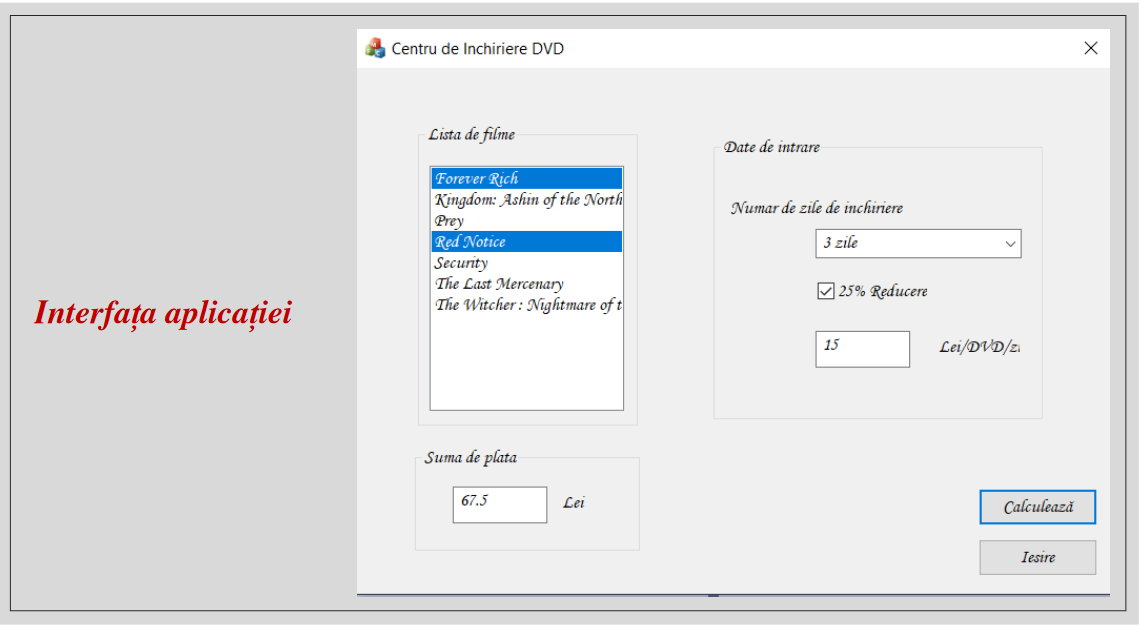
\includegraphics[width=0.60\textwidth]{Imagini/Comune/Interfata.png}
    \caption{Interfața din Cerință}
    \label{fig:mesh1}
\end{figure}



\newpage

\section{Rezolvarea problemei}
\quad Soluționarea temei presupune parcurgerea a două etape:
\begin{itemize}
    
    \item Proiectarea interfeței 
    \item Asigurarea funcționalității
\end{itemize}



\subsection{Proiectarea interfeței aplicației.}
\hfill \newline
Aplicația este de tip \textit{Dialog Base}, elementele sunt separate în patru zone delimitate utilizând \textbf{Group Box-uri}, fiecare cu un nume specific. \:

%%%%%%%%%%%%%%%%%%%%%% IMAGINE COMPLETA

\begin{figure}[h]
    \centering
    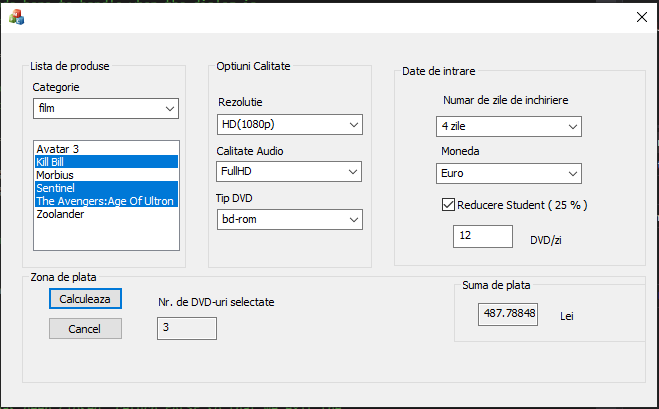
\includegraphics[width=0.60\textwidth]{Imagini/Madaras/FULL.png}
    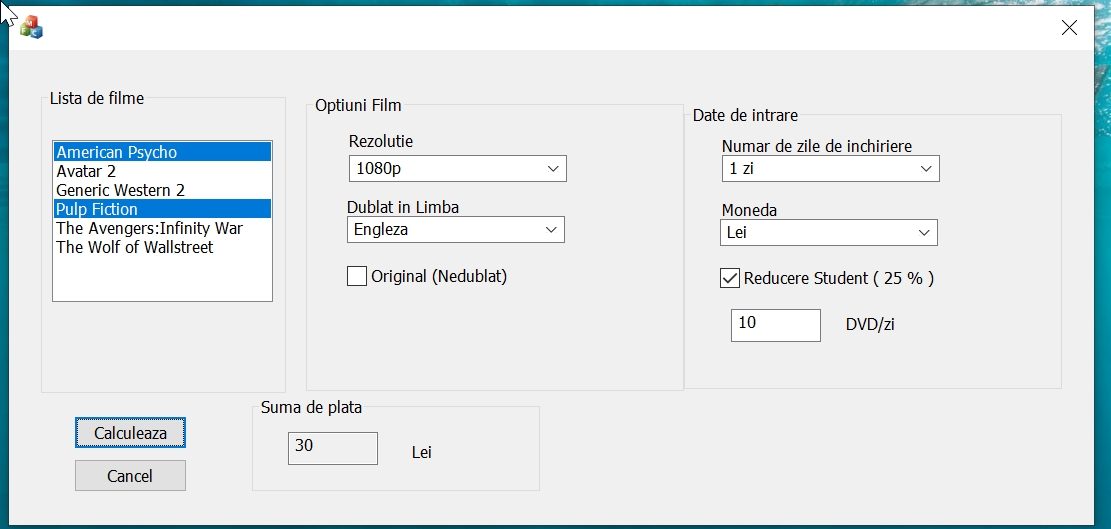
\includegraphics[width=0.60\textwidth]{Imagini/Liviu/Linterfara_plina.jpg}
    \caption{Interfața din Cerință}
    \label{fig:mesh1}
\end{figure}



%%%%%%%%%% AICI SUNTEM  LISTA DE PRODUSE %%%%%%%%%%%%%%%%%%%%%%%%%%%%%%%%%%%%%%%%%%%%%%%%%%%

\subsubsection{\textbf{Lista de produse}}\hfill
\newline 
Zona denumită \textit{Listă de produse} este proiectată pentru a oferii utilizatorului posibilitatea de a alege dintre mai multe * { categorii de fișiere , aplicația punând accent pe filme , opțiunile fiind : }

%%%%%%%%%%%%%%%%%%%%%%%%%%%%%%%%%%%%%%%%%%%%%%%%%%%%%%%%%
%%!LIVIU
% Zona denumita \textit{Lista de filme} este proiectata pentru a oferii utilizatorului o list cu diverse filme { Avatar2, Generic Western 2 , etc.. }
%

Zona denumită \textit{Date de intrare} lasă utilizatorul să selecteze datele de plată pentru închiriere. Această consistă dintre un \textbf{Combo Box}  numit \textit{Număr de zile închiriate} care te lasă să selectezi numărul de zile pentru închirierea filmului și un alt \textbf{Combo Boxl} numit \textit{Monedă} care te lasă să selectezi moneda dorită. De asemenea există un \textbf{Radio Button} care aplică o reducere de 25\% dacă utilizatorul este student.





\begin{itemize}
\item Film
\item Video
\item Music
\end{itemize}
    
/ **{filme}
\hfill \newline

Urmând ca mai jos utilizatorul , prin intermediul unui control de tipul \textbf{Combo Box} , să poată să vizualizeze opțiunile sale , putând alege prin efectuarea unui click asupra numelui **{filmului preferat}/*{fișierului preferat}.

%%% aici
\begin{figure}[h]
\centering
\includegraphics[width=0.40\textwidth]{Imagini/Madaras/FILME.png}
\includegraphics[width=0.40\textwidth]{Imagini/Liviu/FILME.jpg}
\caption{Exemplu de opțiuni filme}
\end{figure}
\hfill \newline

\newpage %%%%%%%%%%%%%%%%%%%%%%%%%%%%%%%%%%%%%%%%%%%%%%%%%%%%%%%%%%%%%%%%%%%%%%%%%%%%%%%%%%% OPTIUNI AICI

\subsubsection{\textbf{Opțiuni Calitate}}\hfill
\newline 

Secțiunea numită \textit{Opțiuni Calitate} este concepută pentru a oferi utilizatorului posibilitatea de a alege dintre mai multe opțiuni calitative , selectând una din variantele date în componente , **{filmului}/*{produsului} dorit.
\newline

\begin{enumerate}[label=\arabic*.] 

\item \textit{Rezoluție:} Aflata într-un \textbf{Combo Box} , utilizatorul putând selecta rezoluția dorita asupra **{filmului}/*{filmului sau videoclipului} selectat anterior din lista de produse *{( În plus, dacă utilizatorul va fi selectat un produs muzical la pasul anterior atunci aceasta opțiune va fi ascunsa ; deoarece un produs exclusiv muzical nu va avea aceasta proprietate )
\hfill \newline

\item **{ \textit{Dublat} : Opțiune redata printr-un Radio Button , prin selecția acestuia utilizatorul va opta pentru o versiune dublata a filmului}
\hfill \newline

\item *{\textit{Calitate Audio} : Aflata într-un Combo Box  , utilizatorul va putea selecta astfel calitatea audio a produsului selectat anterior }
\hfill \newline

\item *{\textit{Tip DVD}} : Aflata într-un Combo Box , utilizatorul va putea selecta tipul de DVD pe care produsul va fi encodat}



\end{enumerate}

\hfill \newline

\begin{figure}[h]
\centering
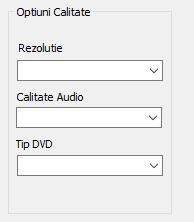
\includegraphics[width=0.40\textwidth]{Imagini/Madaras/OPTIUNI.png}
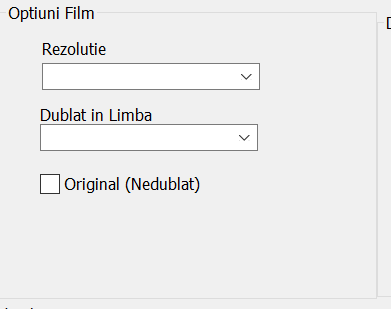
\includegraphics[width=0.40\textwidth]{Imagini/Liviu/OPTIUNI_LIVIU.png}
\caption{Optiunile posibile}
\end{figure}


\hfill \newline

\newpage %%%%%%%%%%%%%%%%%%%%%%%%%%%%%%%%%%%%%%%%%%%%%%%%%%%%%%%%%%%%%%%%%%%%%%%%%%%%%% DATE DE INTRATE AICI


\subsection{Date de Intrare}

Secțiunea denumită "Date de Intrare" oferă utilizatorului noi opțiuni de customabilitate , în sensul alegerii monedei de plata pentru închirierea unui DVD. cu produsul respectiv , selectarea reducerii de student cat și numărul de zile pe care va/vor fi închiriat/e, cat și numărul în sine de DVD.-uri.

\hfill \newline

Funcționalitatea fiind redata prin : 

\hfill \newline

\begin{enumerate}[label=\arabic*.]
\item Lista "Număr de zile de închiriere" : Combo Box cu mai multe opțiuni pentru numărul de zile

\hfill \newline

\item Lista "Moneda": Combo Box cu doua opțiuni pentru moneda asociata prețului nominal mediu al unui DVD.

\hfill \newline

\item Butonul "Reducere Student" : Radio Button prin care se aplica o reducere de 25% la produse , pe baza ca utilizatorul este student.

\hfill \newline

\item Chenarul "DVD/zi" : Edit Control prin care utilizatorul poate introduce prețul numerar al unui DVD al unui produs închiriat pentru o zi

\hfill \newline


\begin{figure}[h]
\centering
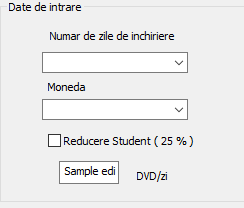
\includegraphics[width=0.40\textwidth]{Imagini/Comune/INTRARE.png}
\caption{Date de intrare}
\end{figure}


\hfill \newline

\end{enumerate}




\hfill \newline

\newpage %%%%%%%%%%%%%%%%%%%%%%%%%%%%%%%%%%%%%%%%%%%%%%%%%%%%%%%%%%%%%%%%%%%%%%%%%%%%%% ZONA DE CALCUL AICI

\subsubsection{\textbf{Zona de plata}}\hfill

Secțiunea denumită \textit{Zona de plata} este concepută pentru a oferi utilizatorului posibilitatea de a vedea atât numărul de produse selectate cat și de a calcula și afișa suma totala de plata pentru produsul cu opțiunile și prețul ales.

\hfill \newline

În componenta acesteia se regăsesc :

\hfill \newline

\begin{enumerate}[label=\arabic*.]
\item Butonul intitulat \textit{Calculeaza}: Componenta de tipul \textbf{Button Control}, oferă utilizatorului funcționalitatea de a calcula suma totala de plata , ca apoi aceasta sa apară în chenarul \textit{Suma de plata}
\hfill \newline

\item Butonul intitula \textit{Cancel}: Componenta de tipul \textbf{Button Control} , oferă utilizatorului opțiunea de a închide și salva cele scrise în aplicație , varianta mai rapida apăsării pe butonul "X" din bara de titlu a aplicației 
\hfill \newline

\item Chenarul \textit{Nr. DVD selectate}: Componenta de tipul \textbf{Edit Control} , componenta prin care utilizatorul poate vizualiza cate produse a selectat
\hfill \newline

\item Sub-secțiunea \textit{Suma de plata}: Componenta de tipul \textbf{Edit Control} , componenta prin care utilizatorul poate vizualiza suma pe care va trebuii sa o plătească pentru produsele selectate în lei
\hfill \newline


\begin{figure}[h]
\centering
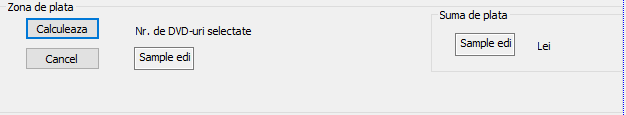
\includegraphics[width=0.80\textwidth]{Imagini/Comune/PLATA.png}
\caption{Zona de plata}
\end{figure}


\hfill \newline

\end{enumerate}





\newpage %%%%%%%%%%%%%%%%%%%%%%%%%%%%%%%%%%%%%%%% DE AICI IN JOS THE FUN BEGINS ( COD )


%%%%%%%%%%%%%%%%%Jesse : CODE, b/itch !

\subsection{Asigurarea funcționalității aplicației}
\hfill \newline

În aceasta secțiune este explicat și prezentat codul visual c++ necesar funcționarii aplicației. 
\hfill \newline

Fișierul de tip .h (header), ce conține prototipurile funcțiilor și genericelor folosite în aplicație 
\hfill \newline


\begin{lstlisting}[language=C++]{Name=test2}
// Lab4Dlg.h : header file
//

#pragma once


// CLab4Dlg dialog
class CLab4Dlg : public CDialogEx
{
// Construction
public:
	CLab4Dlg(CWnd* pParent = nullptr);	// standard constructor

// Dialog Data
#ifdef AFX_DESIGN_TIME
	enum { IDD = IDD_LAB4_DIALOG };
#endif

	protected:
	virtual void DoDataExchange(CDataExchange* pDX);	// DDX/DDV support


// Implementation
protected:
	HICON m_hIcon;

	// Generated message map functions
	virtual BOOL OnInitDialog();
	afx_msg void OnSysCommand(UINT nID, LPARAM lParam);
	afx_msg void OnPaint();
	afx_msg HCURSOR OnQueryDragIcon();
	DECLARE_MESSAGE_MAP()
	LONG NR_DVD;
public:
	CListBox Lista;
	CString Moneda;
	CComboBox Zile;
	CComboBox moneda;
	CComboBox recording_type;
	CComboBox calitate_Audio;
	CComboBox calitate_Film;
	CComboBox categorie;
	CComboBox ComboList[6];
	CString REZOLUTIE;
	BOOL Reducere;
	long Pret;
	double Total;
	double Total_DVD;
	CString Text_Lei;
	afx_msg void OnBnClickedCalculeaza();
	afx_msg void OnLbnSelchangeList();
	afx_msg void OnBnClickedReducere();
	afx_msg void OnCbnSelchangeCombo2();
	CButton s;
	afx_msg void OnStnClickedStatic6();
	afx_msg void OnEnChangeTotal();
	afx_msg void OnStnClickedStatic3();
	afx_msg void OnCbnSelchangeCombo();
	afx_msg void OnStnClickedStatic35();
	afx_msg void OnStnClickedMoneda();
	afx_msg void OnCbnSelchangeCombo6();
	afx_msg void OnCbnSelchangeCombo5();
	afx_msg void OnCbnSelchangeCombo3();
	afx_msg void OnCbnSelchangeCombo4();
	afx_msg void OnEnChangeTotal2();
};



\end{lstlisting}


\newline \hfill

Funcția de tip "Constructor" pentru genericul asociat aplicației de tip dialog MFC cu parametrii necesari



\begin{lstlisting}[language=C++]{Name=test2}


CLab4Dlg::CLab4Dlg(CWnd* pParent /*=nullptr*/)
	: CDialogEx(IDD_LAB4_DIALOG, pParent)
	, Reducere(FALSE)
	, Pret(0)
	, Total(0)
	, Total_DVD(0)
	, Text_Lei(_T(""))
	, Moneda(_T("Lei"))
{	
	m_hIcon = AfxGetApp()->LoadIcon(IDR_MAINFRAME);
}
 \end{lstlisting}


\hfill \newline
\newpage

\begin{lstlisting}[language=C++]{Name=test2}

void CLab4Dlg::DoDataExchange(CDataExchange* pDX)
{
	CDialogEx::DoDataExchange(pDX);
	DDX_Control(pDX, IDC_LIST, Lista);
	DDX_Control(pDX, IDC_COMBO, Zile);
	DDX_Control(pDX, IDC_COMBO2, moneda);
	DDX_Check(pDX, IDC_REDUCERE, Reducere);
	DDX_Text(pDX, IDC_PRET, Pret);
	//DDX_LBString(pDX, IDC_STATIC9, REZOLUTIE);
	DDX_Text(pDX, IDC_TOTAL, Total);
	DDX_Text(pDX, IDC_TOTAL2, Total_DVD);
	DDX_Control(pDX, IDC_COMBO6, categorie);
	DDX_Control(pDX, IDC_COMBO3, calitate_Film);
	DDX_Control(pDX, IDC_COMBO4, calitate_Audio);
	DDX_Control(pDX, IDC_COMBO5, recording_type);
	//DDX_Text(pDX, IDC_MONEDA,Text_Lei);
	
}
 \end{lstlisting}

Funcția ce asigura transmisia de date intre componente și variabilele asociate.
Are loc prin apelarea genericului DDX Control sau celelalte variante în funcție de componenta dând ca parametrii: handle către window : pDX, componenta si variabila

\hfill \newline
\hfill \newline

\newpage


De asemenea voi prezenta codul apropriat secțiunii/subsecțiunii respective. 


\hfill \newline
 Astfel : 
\hfill \newline
\subsubsection{\textbf{Cod Lista de produse}}\hfill

\hfill \newline
\hfill \newline
 Mai jos se regăsește codul asociat generării, selecției unei opțiuni din \textbf{ComboBox} și afișarea lor în \textbf{List Box}  

%%%%%%%%%%%%%%%%%%%%%%%%%%%%%%%%%%%%%%%% COD MADARAS 

\begin{lstlisting}[language=C++]{Name=test2}


  void CLab4Dlg::OnCbnSelchangeCombo6()
{
    
	if (categorie.GetCurSel() == 0)
	{
		while (Lista.GetCount() > 0)
		{
			int i = 0;
			Lista.DeleteString(i);
			i++;
		}
        
		Lista.AddString((LPCWSTR)L"Sentinel");
		Lista.AddString((LPCWSTR)L"Avatar 3");
		Lista.AddString((LPCWSTR)L"The Avengers:Age Of Ultron");
		Lista.AddString((LPCWSTR)L"Morbius");
		Lista.AddString((LPCWSTR)L"Zoolander");
		Lista.AddString((LPCWSTR)L"Kill Bill");

		calitate_Film.ShowWindow(SW_SHOW);
	}



	if (categorie.GetCurSel() == 1)
	{
		while (Lista.GetCount() > 0)
		{
			int i = 0;
			Lista.DeleteString(i);
			i++;
		}

		Lista.AddString((LPCWSTR)L"Popular Video Example");
		Lista.AddString((LPCWSTR)L"Some Video");
		Lista.AddString((LPCWSTR)L"NatGeo elephants video");
		Lista.AddString((LPCWSTR)L"Some Video2");

		calitate_Film.ShowWindow(SW_SHOW);
	}

	if (categorie.GetCurSel() == 2)
	{
		while (Lista.GetCount() > 0)
		{
			int i = 0;
			Lista.DeleteString(i);
			i++;
		}

		Lista.AddString((LPCWSTR)L"Popular Song Example");
		Lista.AddString((LPCWSTR)L"Album 1");
		Lista.AddString((LPCWSTR)L"Animal Sounds");
		
		calitate_Film.ShowWindow(SW_HIDE);

	}


}
 \end{lstlisting}


 \begin{lstlisting}[language=C++]{Name=test2}

BEGIN_MESSAGE_MAP(CLab4Dlg, CDialogEx)
	ON_WM_SYSCOMMAND()
	ON_WM_PAINT()
	ON_WM_QUERYDRAGICON()
	ON_BN_CLICKED(IDC_CALCULEAZA, &CLab4Dlg::OnBnClickedCalculeaza)
	ON_LBN_SELCHANGE(IDC_LIST, &CLab4Dlg::OnLbnSelchangeList)
	ON_CBN_SELCHANGE(IDC_COMBO6, &CLab4Dlg::OnCbnSelchangeCombo6) // ACESTA
	ON_EN_CHANGE(IDC_TOTAL2, &CLab4Dlg::OnEnChangeTotal2)
END_MESSAGE_MAP()

 \end{lstlisting}


\subsubsection{\textbf{Cod Lista de produse}}\hfill

\hfill \newline
\hfill \newline

 


 
\hfill \newline
Funcția redata mai sus este asociata selecției unei opțiuni în \textbf{ComboBox} prin delegarea sa \textit{OnCbnSelchangeCombo6} către namespace-ul oferit aplicației de tip dialog \textbf{CLab4Dlg}ca apoi sa fie mapat folosind metoda "BEGIN MESSAGE MAP" asociata.

 Aplicaților de tip MFC prin linking-ul cu fișierele  de tip .dll specifice.
\hfill \newline
	Funcția se folosește de metode clasice regăsite elementelor de tip MFC precum ("GetCurSel" sau "GetCount") pentru a captura selecția utilizatorului și a itera prin lista de opțiuni cu scopul de a adaugă sau șterge în funcție de selecție. 
 \hfill \newline
 
%%%%%%%%%%%%%%%%%%%%%%%%%%%%%%%%%%%%%%%% COD MADARAS 




%%%%%%%%%%%%%%%%%%%%%%%%%%%%%%%%%%%%%%%% COD LIVIU
 

 \begin{lstlisting}[language=C++]{Name=test2}

BEGIN_MESSAGE_MAP(CLab4Dlg, CDialogEx)
	ON_WM_SYSCOMMAND()
	ON_WM_PAINT()
	ON_WM_QUERYDRAGICON()
	ON_BN_CLICKED(IDC_CALCULEAZA, &CLab4Dlg::OnBnClickedCalculeaza)
	ON_LBN_SELCHANGE(IDC_LIST, &CLab4Dlg::OnLbnSelchangeList)
	ON_CBN_SELCHANGE(IDC_COMBO6, &CLab4Dlg::OnCbnSelchangeCombo6) // ACESTA
	ON_EN_CHANGE(IDC_TOTAL2, &CLab4Dlg::OnEnChangeTotal2)
END_MESSAGE_MAP()

\end{lstlisting}

\hfill \newline
    Funcția redata mai sus este asociata selecției unei opțiuni în \textbf{ComboBox} prin delegarea sa \textit{OnCbnSelchangeCombo6} către namespace-ul oferit aplicației de tip dialog \textit{CLab4Dlg}
	ca apoi sa fie mapat folosind metoda "BEGIN MESSAGE MAP" asociata Aplicaților de tip MFC prin linking-ul cu fișierele  de tip .dll specifice.

\hfill \newline


	Funcția se folosește de metode clasice regăsite elementelor de tip MFC precum ("GetCurSel" sau "GetCount") pentru a captura selecția utilizatorului și a itera prin lista de opțiuni cu scopul de a adaugă sau șterge în funcție de selecție. 
 \hfill \newline

%%%%%%%%%%%%%%%%%%%%%%%%%%%%%%%%%%%%%%%% COD LIVIU

\newpage
%%%%%%%%%%%%%%%%%%%%%%%%%%%%%%%%%%%%%%%%% COD PLATA

\subsubsection{\textbf{Zone de Plata}}\hfill

\hfill \newline
\hfill \newline

Mai jos se regăsește codul asociat calculului sumei totale.

\hfill \newline


 \begin{lstlisting}[language=C++]{Name=test2}

 void CLab4Dlg::OnBnClickedCalculeaza()
{
	
	UpdateData();


	if (Zile.GetCurSel() == CB_ERR)
		Zile.SetCurSel(0);
	if (moneda.GetCurSel() == CB_ERR)
		moneda.SetCurSel(0);
	if (categorie.GetCurSel() == CB_ERR)
		categorie.SetCurSel(0);
	if (calitate_Film.GetCurSel() == CB_ERR)
		calitate_Film.SetCurSel(0);
	if (calitate_Audio.GetCurSel() == CB_ERR)
		calitate_Audio.SetCurSel(0);
	if (recording_type.GetCurSel() == CB_ERR)
		recording_type.SetCurSel(0);


	DOUBLE Fhd = 1;
	DOUBLE Shd = 1;
	DOUBLE ZileSale = 1;
	if (calitate_Film.GetCurSel() == 3)
		Fhd = 1.5; 
	if (calitate_Film.GetCurSel() == 4)
		Fhd = 2;

	if (recording_type.GetCurSel() == 1)
		Shd = 1.5;

	if (Zile.GetCurSel() >= 1)
		ZileSale = 0.6;

	if (moneda.GetCurSel() == 0) {
		Total = ((DOUBLE)Zile.GetCurSel() + 1) *ZileSale * Pret * (DOUBLE)Lista.GetSelCount() * ( ((DOUBLE)calitate_Film.GetCurSel()+1) * 0.34) * Fhd *
			(((DOUBLE)calitate_Audio.GetCurSel()+1) * 0.5) * ((DOUBLE)recording_type.GetCurSel()+1) * Shd  * (Reducere ? 0.75 : 1);
		
	}
	else {

		Total = ((DOUBLE)Zile.GetCurSel() + 1) * ZileSale * Pret * (DOUBLE)Lista.GetSelCount() * (((DOUBLE)calitate_Film.GetCurSel() + 1) * 0.34) * Fhd *
			(((DOUBLE)calitate_Audio.GetCurSel() + 1) * 0.5) * ((DOUBLE)recording_type.GetCurSel() + 1) * Shd * (Reducere ? 0.75 : 1) * 4.92;
		
	}
	UpdateData(FALSE);

Text_Lei = "Lei";
UpdateData(TRUE);

}

 \end{lstlisting}

Funcția redata mai sus este asociata selecției unei opțiuni în ComboBox prin delegarea sa ("OnBnClickedCalculeaza") către namespace-ul oferit aplicației de tip dialog (CLab4Dlg) ca apoi sa fie mapat folosind metoda "BEGIN MESSAGE MAP" asociata Aplicaților de tip MFC prin linking-ul cu fișierele  de tip .dll specifice.

\hfill \newline

Funcția se folosește de metode clasice elementelor din MFC pentru a calcula suma totala de plata în funcție de toate opțiunile regăsite în aplicație, selectate sau modificate de către utilizator. 

\hfill \newline

\subsubsection{Astfel} : 
\hfill \newline

\begin{enumerate}[label=\arabic*.]
\item "Zile.GetCurSel()": se refera la selecția unei zile (folosit în ecuație pentru a  rezulta 0 dacă utilizatorul nu a selectat nimic)
\hfill \newline

\item "ZileSale" : se refera la numărul de zile selectate
\hfill \newline

\item "Preț" : se refera la prețul unui DVD
\hfill \newline

\item \textbf{ "Lista.GetSelCount()" : se refera la numărul asociat selecției de calitate , acesta este înmulțit cu   calitateFilm.GetCurSel() + 1  
pentru a simula o creștere treapta în preț (opțiunea "4k" costând de 8 ori cat prima)}

\end{enumerate}

\hfill \newline
Funcția UpdateData(paramentu) trimițând un semnal către MFC pentru a updata datele din vederea utilizatorului.





\newpage

% lucrarile incluse in bibliografie se citeaza obligatoriu in textul lucrarii
% folosind comanda \cite
\newpage
\hfill \newline
\hfill \newline

\centerline{Va mulțumesc pentru atenție !}   

\hfill \newline
\hfill \newline
\hfill \newline


\begin{thebibliography}{99}
\bibitem{link1} \url{https://learn.Microsoft.com/en-us/cpp/mfc/mfc-desktop-applications?view=msvc-170}
\bibitem{link1} \url{https://learn.microsoft.com/en-us/cpp/mfc/message-handling-and-mapping?view=msvc-170}
\bibitem{link1} \url{https://https://learn.microsoft.com/en-us/cpp/mfc/mfc-application-architecture-classes?view=msvc-170}
\bibitem{link1} \url{https://www.functionx.com/visualc/}
\bibitem{link1} \url{https://depts.washington.edu/cmmr/biga/chapter_tutorial/1.C++_MFC_D3DOGL/1.StepByStepGuide/tutorial_1.html}
\end{thebibliography}




\end{document}

